\begin{fullwidth}
    \section{Markets} \label{sec:markets}

    \begin{adjustwidth}{2cm}{2cm}
        \justify
        dYdX v4 empowers the community to control market listings and market parameters through on-chain governance proposals. The timely listing of new markets is a crucial component of growth in the fast-paced industry of decentralized finance, and requires sophisticated risk-management to ensure market parameters reflect the risks of underlying tokens. Furthermore, dYdX v4 will eventually launch a permissionless listings program, which will enable any user to list a new market by specifying its oracle, market parameters, and perhaps providing some initial liquidity. In this section we discuss initial market listings for dYdX v4, the community's responsibility in listing new markets and managing market parameters, and a few thoughts on permissionless listings design. The permissionless listings ideas presented here are the product of discussions with several community members at dYdX, and other DeFi protocols including Osmosis.
    \end{adjustwidth}
    
    \textcolor{gray}{\rule{\linewidth}{0.1mm}}

\end{fullwidth}

    \subsection{Market Listings Overview} \label{subsec:markets}

        Listing new markets, closing existing markets, and updating market parameters are all done via governance proposals on dYdX v4. This entails a large responsibility for the dYdX community to vote on market listing proposals and ensure market parameters are kept up to date with market trends and liquidity.

        To service these responsibilities, the dYdX community may choose to establish a dedicated markets subDAO, or onboard sophisticated service providers.

        \subsubsection{Initial Market Listings}

            dYdX v4's initial markets are displayed in Appendix \ref{appsubsec:perps}, and are largely based on the successful markets of dYdX v3. These include BTC, ETH, OP, LINK, as well as newer tokens such as WLD, BLUR, and PEPE. 

        \subsubsection{Market Parameters}
    
            Each market listing carries with it a few market parameters, including:

            \begin{itemize}
                \item \textbf{Tick sizes:} The smallest change in market prices considered by the exchange.
                \item \textbf{Oracle:} The source[s] of a market's underlying spot price, such as Binance, OKX, or other spot exchanges.
                \item \textbf{Liquidity Tiers:} The liquidity tier a market belongs to, either small cap, mid cap, or large cap. These liquidity tiers are appointed on a discretionary basis, and determine the minimum and maintenance margin requirements for positions held in the market, among other things.
            \end{itemize}

            The market parameters for the ETH market on dYdX v3 are depicted in Fig. \ref{fig:eth_mkt_params}.

            \begin{figure}[htp]
                \centering
                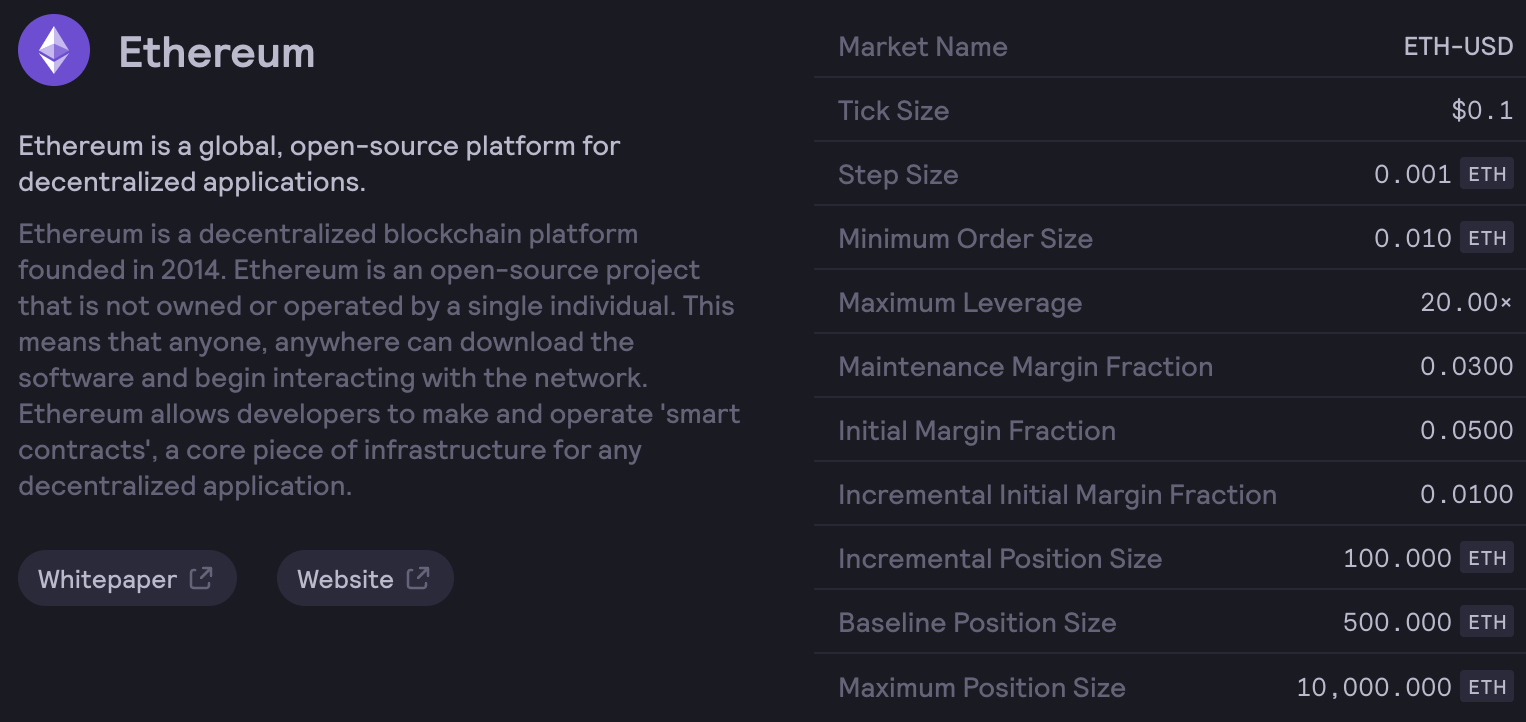
\includegraphics[width=\linewidth]{figs/ETH_mkt_params.png}
                \captionsetup{width=\linewidth}
                \caption{ETH market parameters for dYdX v3.}
                \label{fig:eth_mkt_params}
            \end{figure}

        \subsubsection{Market Risks}

            All three market parameters outlined previously-tick sizes, oracles, and liquidity tiers-are crucial in maintaining a healthy derivatives exchange. Tick size width affects the liquidity profile of different markets, and affects the profitability of both makers and takers on the exchange. Oracles are crucial for reporting accurate prices; in the worst-case scenario, a user listing a malicious oracle could sway prices in their favor, causing financial harm to all traders taking the other side of the user's position. Finally, liquidity tiers are key for determining margin requirements, which themselves are a highly sensitive parameter. Setting margin requirements too high can be stifling for traders, encouraging them to trade on alternative derivatives exchanges where they can acquire more leverage. Alternatively, low margin requirements can lead to unprofitable or missed liquidations if there is insufficient liquidity to close underwater positions.

            Ensuring these parameters are set appropriately is a challenging task. Community members or service providers must monitor positions and tune parameters according to shifting market forces. If a certain market becomes less liquid, for example, it might be appropriate to raise its margin requirement, and vice-versa. 

    \subsection{Permissionless Markets} \label{subsec:corepermissionless}
    
        \textit{Disclaimer: This discussion is the product of several conversations with community members at dYdX and the broader Cosmos ecosystem; it makes a few assumptions regarding the design of dYdX Chain.}

        Under a permissionless listings paradigm, any market can be listed, with any oracle, and any set of market parameters. Of course, the community may choose to enforce boundaries on parameters, or require that oracles originate from certain whitelisted oracle providers such as Chainlink.\sidenotequote{Permissionless pool creation, within Governance permissioned boundaries, interacted with through permissioned frontends}{\bhref{https://twitter.com/JohnnyWyles87}{Johnny Wyles}, governance lead at Osmosis, on Osmosis' permissionless listings paradigm.} This permissionless paradigm allows anyone to identify new and attractive markets and list them on dYdX, bringing additional supply and demand to the exchange. This might meaningfully improve dYdX's ability to capture new and emerging markets, acquiring new users and increase dYdX's overall market share in the derivatives space. 
        
        To that end, permissionless listings have been successful components of growing many AMMS, most notably Uniswap and Osmosis. Uniswap in particular observed significant growth over the last several years due to its ability to quickly onboard new pools, and capture that market share.

        \begin{figure}[htp]
            \centering
            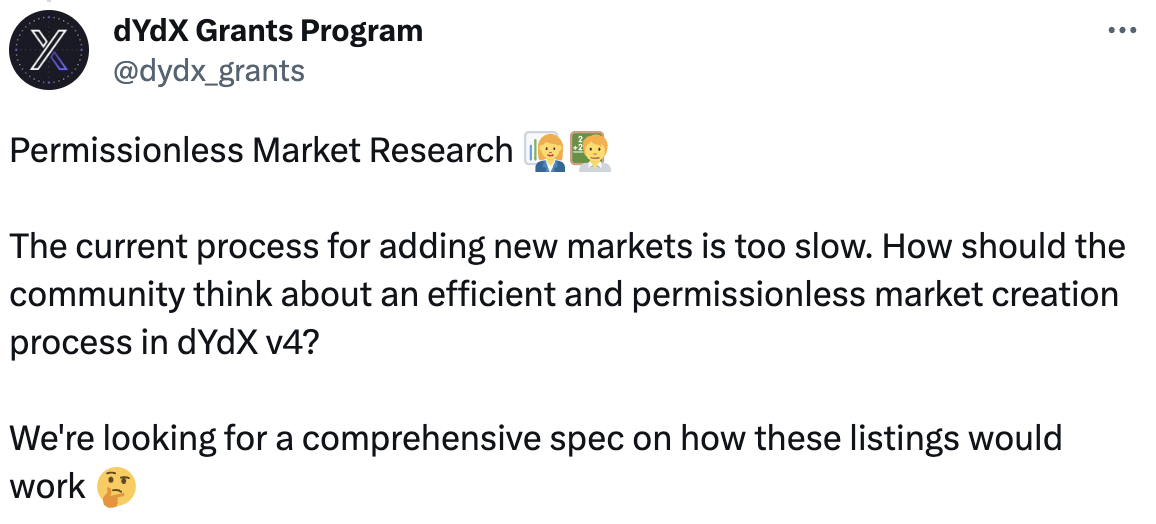
\includegraphics[width=0.7\linewidth]{figs/dgp_pl.png}
            \captionsetup{width=0.7\linewidth}
            \caption{dYdX Grants Program's \bhref{https://x.com/dydx_grants/status/1638526591004180481?s=20}{Tweet} on Permissionless Listings Research.}
            \label{fig:dgp_tweet}
        \end{figure}
        
        However, permissionless listings might also create incentives for listing ``malicious markets'', where the entity listing the market controls either the oracle or the supply of the underlying token. Furthermore, permissionless listings allow the same underlying token to be listed over several markets, fragmenting liquidity for long-tail assets. We wish to mitigate all these effects with the sound design of a permissionless listings framework. The first step in doing so is to distinguish between \textit{permissionless markets} and \textit{core markets}. 

        \textit{We will refer to those listing permissionless markets as Sponsors}.
            
        \subsubsection{Core and Permissionless Markets}

            Permissionless markets have few security assumptions; traders must be cautious of potential scams or attacks. These markets are similar to the ``unverified'' pools listed on \bhref{https://frontier.osmosis.zone}{Osmosis Zone}\sidenote{Unverified pools on Osmosis were previously listed on Osmosis Frontier instead. On September 2023, Osmosis Frontier was merged with Osmosis Zone, the primary Osmosis front end, to consolidate and simplify the user experience.}. Core markets, on the other hand, have either been listed by governance or were previously permissionless markets that have since been upgraded. dYdX may choose to distinguish between core and permissionless markets both in terms of the user experience, and in terms of the protocol's various liquidation and incentives mechanisms:
    
            \begin{enumerate}
                \item \textbf{UX:} Provide clarity for front ends operators on how they might prioritize the display of different markets. For example, \bhref{https://osmosis.zone/}{Osmosis Zone} allows users to hide permissionless markets using a simple toggle button. Alternatively, permissionless markets might be displayed on separate tabs or separate front ends entirely, as used to be the case with Osmosis Frontier.
                \item \textbf{Incentives, Insurance, and Margin:} Permissionless markets might be subject to a number of inefficiencies or malicious attacks, discussed below. To avoid the risk of contagion, we might isolate permissionless markets from the rest of the protocol. For example, we might launch permissionless markets with isolated margin and insurance funds.
            \end{enumerate}
    
            \begin{figure*}
                \centering
                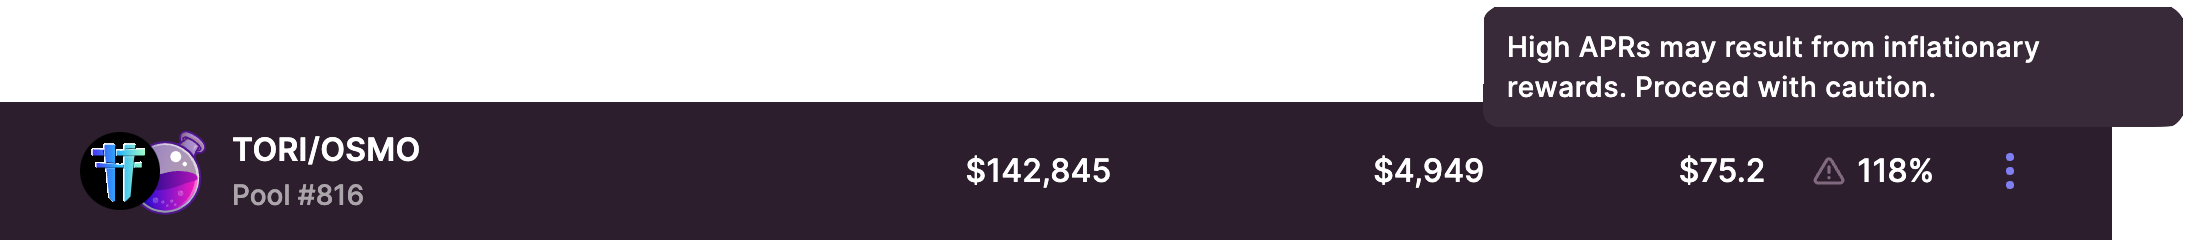
\includegraphics[width=\linewidth]{figs/frontierwarning.png}
                \captionsetup[]{width=\linewidth}
                \caption{High APR warning on Osmosis, a tool to prevent retail LPs from falling for scams. Note: we are not making any statement about the token being depicted in this figure.}
                \label{fig:frontierwarning}
            \end{figure*}


    \subsection{Permissionless Market Risks}

        To motivate the discussion for designing permissionless listings, we first discuss some of the associated risks. Particularly, we consider how permissionless listings may be leveraged to attack or scam dYdX users using tampered oracles or tampered token supplies. Furthermore, we consider how permissionless listings might fragment liquidity across the exchange.

        \subsubsection{Tampered Market Listings}

            Consider Osmosis, one of the most successful application chains on Cosmos. Osmosis launched a permissionless listings program along with a permissionless incentives program. Permissionless incentives enabled the team listing a new pool to incentivize liquidity, at no additional cost to the Osmosis treasury or OSMO inflation. It also, however, enabled malicious actors to list pools for obscure projects with enourmous incentives. This lead to several pools being listed with APRs in the 100\%+ range, indicating that one of the tokens in the pool has a highly inflationary schedule. Liquidity providers are then tricked into LP'ing into the pool to grab some of the APR. To do so they must purchase a large quantity of the underlying token, at which point the malicious sponsor ``rugs'' the project by market selling a large portion of the circulating supply.

            Osmosis has considered several approaches to mitigating the damage from malicious listings, some of which are discussed later in this section. One mitigation tool is a listing fee (currently at 100 OSMO), as well as several cosmetic approaches to warn retail users browsing the Osmosis Zone front end that astronomical APRs are indicative of potential scams, shown in Figure \ref{fig:frontierwarning}. See  \bhref{https://commonwealth.im/osmosis/discussion/11255-minimising-scam-pools}{this} forum post for the ongoing discussion on Osmosis.\sidenotequote{A review of the last 80 liquidity pools created (Pool \#938 through Pool \#1018, which are roughly all those that have been created since the beginning of March), \textbf{found that 55 of them (or 80\%) to be either scam, spam, or, predatory}.}{\bhref{https://forum.osmosis.zone/t/proposals-addressing-scam-pools-increase-the-pool-creation-fee/42/4}{Osmosis Forums: Proposals Addressing SCAM Pools}}
            
            However, these approaches have a few shortcomings:
            
            \begin{itemize}
                \item Potential gains from successful attacks can far exceed the fixed listing fee.
                \item Cosmetic additions to the UI may not be adopted by all front ends if front ends are decentralized.
                \item Cosmetic additions to the UI often rely on some threshold conditions such as APRs above 75\% being flagged; malicious actors can identify these conditions and subvert them.
            \end{itemize}
            
            The line between mitigating malicious attacks and stifling the growth of permissionless listings is a thin one. Let's first consider some of the potential attacks that might be levied via permissionless listings.

            \textbf{Oracle Manipulation}

            The Sponsor lists a new market with an oracle feed that they control. They may then take a LONG or SHORT position on the market, and change the oracle price to benefit them. They may profit from this manipulation either by earning the funding rate, or by closing their position at a profit as traders exit the market.

            \textbf{Token Supply Manipulation}

            Similar to Oracle manipulation, a sponsor might list a market for a token for which they control a large portion of the supply. This sponsor may then short the perpetual, and conduct a firesale of the token on relevant spot exchanges. As the spot price of the token falls, the sponsor profits from their short position.

            \textbf{Denial-of-Service Attacks and Spam}

            A less pernicious attack is spamming the network with permissionless markets. This might be done maliciously to damage the user-experience for permissionless listings and increase the costs of operating the chain. It might also be a consequence of a low barrier to list markets. For this reason, Osmosis and other permissionless protocols implement listing fees to deter users from spamming new markets.

        \subsubsection{Liquidity Fragmentation}

            Aside from potential scams or attacks on permissionless markets, we must consider the possibility that perpetuals liquidity for underlying tokens becomes fragmented. On dYdX v3 there is exactly one market for each token, with parameters being optimized largely by dYdX Trading. Under a permissionless listings paradigm, there might be several markets for the same token, some with different oracles, different tick sizes, etc.. \sidenotequote{We document significant liquidity fragmentation in 32 out of 242 asset pairs in our sample, which account for 95\% of liquidity committed to Uniswap v3 smart contracts and 93\% of trading volume. For each of the fragmented pairs, trading consolidates on two pools with adjacent fee levels: either 1 and 5 basis points (e.g., USDC-USDT), 5 and 30 basis points (ETH-USDC), or 30 and 100 basis points (USDC-CRV).}{ \textit{Liquidity fragmentation on decentralized exchanges}, by \bhref{https://arxiv.org/pdf/2307.13772.pdf}{Lehar et al., \cite{lehar2023liquidity}},}

            \begin{figure}[htp]
                \centering
                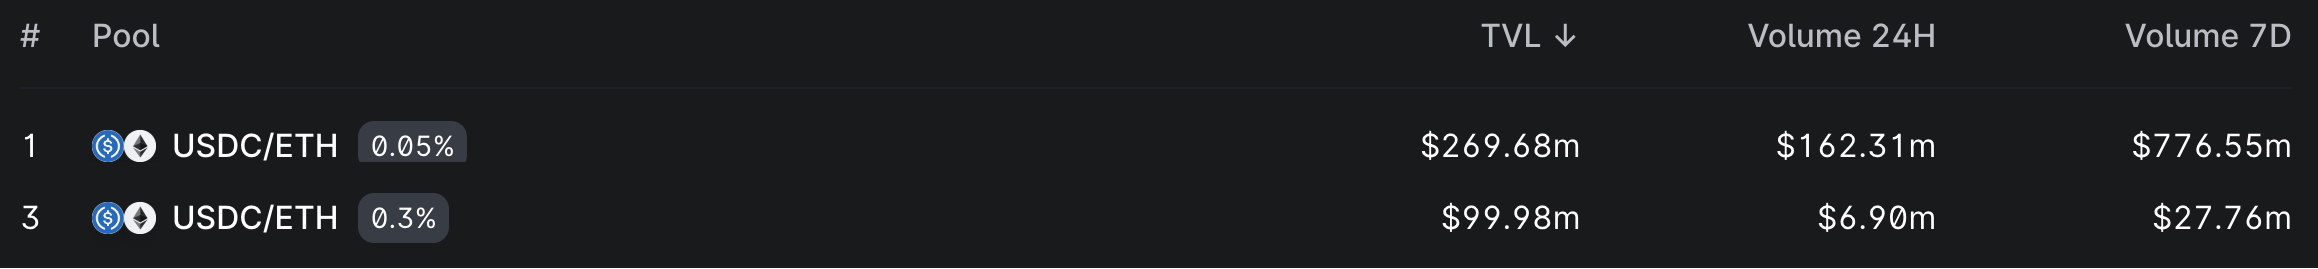
\includegraphics[width=\linewidth]{figs/fragmentation.png}
                \captionsetup{width=\linewidth}
                \caption{Liquidity fragmentation in the Uniswap v3 market for the USDC/ETH pair. Notice that around 27\% of the TVL is held in the higher fee market. Snapped from the Uniswap user interface on August 9th, 2023.}
                \label{fig:fragmentation}
            \end{figure}

            There have been several studies on the fragmentation of liquidity on permissionless AMMs like Uniswap, where different fee and tick sizes attract different profiles of Liquidity Providers. Lehar et al. \cite{lehar2023liquidity} found that large LPs tend to focus on pools with lower fees, where they observe more demand and therefore accrue more fees. Simultaneously, this incurs a number of fixed costs as these LPS must rebalance their positions and pay corresponding gas. Smaller LPs, for whom fixed rebalancing costs like gas fees, tend to concentrate on pools with higher fees and lower trading volume. As demand eats away at the liquidity on lower fee pools, orders begin to be routed to pools with higher fees. This ``economy of scale'' effect causes liquidity fragmentation.

            As we will discuss, upgrading permissionless markets to core markets might help consolidate liquidity for particular tokens on dYdX v4. This signals to makers and takers that this market has additional security assumptions, such as reasonable tokenomics and oracles for the underlying token. Permissionless markets might then be an experimentation phase, where market forces determine which are the best parameters for particular markets, before governance decides which one[s] to upgrade.
            
            However, this does not avoid the fact that some makers and takers might prefer markets with different parameters, and that different equilibria might arise between an XYZ-PERP market with a small tick size, and an XYZ-PERP market with a large tick size. A natural question might then be: how will makers and takers optimally route their orders between numerous potential markets with different parameters?

            \begin{marginfigure}
                \centering
                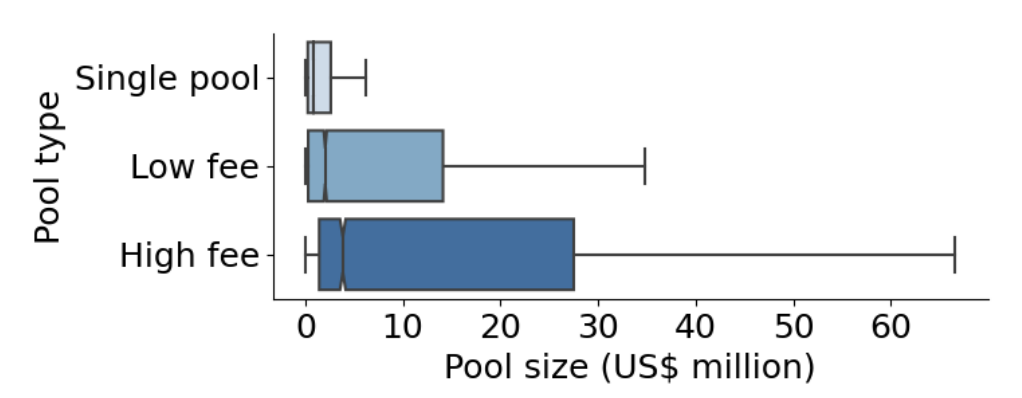
\includegraphics[width=\linewidth]{figs/sizes.png}
                \captionsetup{width=\linewidth}
                \caption{Box plot for empirical data on Uniswap v3 pools by Lehar et al. \cite{lehar2023liquidity}. The plot shows that, for pools with a low fee and high fee option (e.g. 30 bps vs 100bps), the high fee pools observe significantly more liquidity, with this discrepancy being exacerbated for larger pools.}
            \end{marginfigure}


        \subsection{Designing Permissionless Listings}

            We now overview some simple design considerations for permissionless listings with two key objectives in mind:

            \begin{itemize}
                \item \textbf{Growth:} Permissionless listings should foster growth on dYdX v4, this might be done by enabling external incentives, and making the listing process as friction-free as possible.
                \item \textbf{Isolation:} Given their inherent risks, the community might choose to prevent permissionless markets from integrating with protocol-wide mechanisms, such as cross-margining or the liquidation insurance fund.
            \end{itemize}
            
            Whether these considerations do or do not come to fruition on the final design of the permissionless listings program will depend on dYdX Chain governance. We outline them in this report to inform the reader on the various tools at dYdX's disposal to minimize risks and losses to dYdX users.
            
            \subsubsection{Isolated Margining}
                \bhref{https://help.dydx.exchange/en/articles/4797405-how-does-cross-margining-work-on-perpetuals}{Cross margining} allows margin traders to deposit collateral that is shared across multiple positions. This means a trader might deposit 1,000 USDC, and use it to open a LONG BTC-PERP position worth 10,000 USDC, and a SHORT ETH-PERP position worth 10,000 USDC, placing their overall leverage at the 20x maximum. If both BTC and ETH appreciate in value, then the user can offset their losses on their SHORT ETH position against their gains on their LONG BTC position. Without cross-margining, the user might get liquidated on the SHORT ETH position despite gains in their LONG BTC position. On dYdX v3, cross-margining was enabled by default, with isolated margining being possible using sub-accounts.
    
                A concern with permissionless markets is contagion due to cross margining: a user might have several healthy positions open in core markets, and one risky position in a permissionless market. If the permissionless market experiences an oracle attack, then the user might be liquidated, which could affect their positions in other markets. To avoid cascading liquidations between permissionless markets and core markets, we might require all permissionless market positions be made with isolated collateral. This could be done, for example, by using the sub-accounts infrastructure.

        \subsubsection{Liquidation Insurance}
        
            On dYdX v3, price movements lead to unprofitable or missed liquidations on dYdX, the negative balance is discounted from a protocol-wide insurance fund. Similarly, excess profits from timely liquidations count towards the \bhref{https://help.dydx.exchange/en/articles/4797401-perpetual-contract-liquidations}{global insurance fund}. Assuming a similar structure exists for dYdX v4, a natural question is whether unprofitable liquidations on permissionless markets should be discounted from the global insurance fund.

            Like enabling cross margining, enabling the global insurance fund on permissionless markets could create contagion between permissionless markets and core markets. Consistent scams and attacks on permissionless markets might deplete the insurance fund, hampering the ability of liquidators (e.g. the protocol's validators) from performing unprofitable liquidations, leading to missed liquidations and the accrual of ``bad debt''. Due to minimal security assumptions on permissionless markets, dYdX governance might choose to remove them from the global insurance fund entirely.
            
        \subsubsection{External Incentives}

            % dYdX Trading, has recently announced a novel Trader Rewards program for dYdX v4, which we discuss in Section \ref{sec:incentives}. In designing permissionless markets, we might ask whether permissionless markets share in protocol-wide (internal) incentives programs.

            % As it stands, Trader Rewards are disbursed pro-rata based on the amount of fees paid by each user, regardless of which market the fee was paid on. As we discuss in later sections, modifying the Trader Rewards logic to account for the markets an address has interacted with might enable a number of interesting optimizations. One of them is to potentially exclude fees paid on permissionless markets from the rewards calculation. But why would we do that? Fees paid on permissionless markets are still valuable in securing dYdX chain, and due to the new mechanism for distributing trading rewards, they can no longer be ``farmed'' by sophisticated traders\sidenote{Xenophon Labs had \bhref{https://xenophonlabs.com/papers/dydx_trade_rewards.pdf}{previously identified} a dominant Nash Equilibrium for traders to profitably farm the v3 Trader Rewards function. This was possible since the USD value paid out in rewards could \textit{exceed} the USD amount paid in fees. With the new mechanism designed by dYdX Trading, this is no longer possible.}. Disabling trader rewards on permissionless markets would make trading on those markets more expensive, and hamper growth on the very markets where growth is most important! Since fees paid on any market contribute equally to the security of dYdX chain, we might consider maintaining trader rewards on permissionless markets. For similar reasons, we might consider maintaining market maker rebates for permissionless markets as well.
            
            As discussed in Section \ref{sec:validators}, the LP rewards program popularized on dYdX v3 is being discontinued in favor of a market maker rebate program. However, we may consider the implementation of an External Incentives program similar to those implemented on Osmosis. 
            
            Xenophon Labs has previously discussed how LP rewards might be brought ``fully on-chain'' in a \bhref{https://xenophonlabs.com/papers/dydx_token_design_app_layer_incentives.pdf}{previous report}, by modifying the rewards formula to be based exclusively on volume. Assuming the necessary logic were implemented in the dYdX chain codebase, the community may consider enabling the sponsors of any market to include a stream of tokens to be regularly emitted as rewards, both to traders and liquidity providers in their specific permissionless market.

            For example, Sponsor A is interested in listing a market for XYZ-PERP on dYdX v4. Perhaps, Sponsor A is the development team behind token XYZ, or the corresponding DAO, and they believe that perpetuals trading on their token will improve visibility, price discovery, and liquidity on their new token. With that in mind (and perhaps following a governance vote on the XYZ DAO), Sponsor A lists XYZ-PERP, and in that process locks 1M XYZ token to be disbursed as trading rewards and an additional 1M XYZ token to be emitted as volume-based LP rewards for the XYZ-PERP market over the course of 6 months. In that time, the additional trading incentives encourage traders to open positions on XYZ-PERP, and encourages existing market makers to provide the necessary liquidity in that new market. This avoids Sponsor A from having to solicit over-the-counter (OTC) deals with market makers to provide liquidity for their new project, and enables them to stimulate initial trading activity for their derivative.
            
        \subsubsection{Upgrading Markets}

            Ideally, permissionless markets are quickly upgraded to core markets once they achieve a certain amount of popularity. Once upgraded, traders and market makers get to enjoy the benefits of cross-margining, global liquidation insurance, and the additional security assumptions that the oracles and tokenomics for the underlying token are sound. Furthermore, core markets might help consolidate liquidity, and avoid retail users from being scammed.

            To that effect, we might consider two paradigms for quickly upgrading permissionless markets to core markets:

            \begin{enumerate}
                \item \textbf{Automated:} Markets are automatically upgraded to core markets once certain performance thresholds are met, such as a critical amount in 30d volume or open interest.
                \item \textbf{Supervised:} Markets that meet certain performance thresholds are put up for review, and the DAO (or a dedicated subDAO), follows a streamlined process to vote on an upgrade.
            \end{enumerate}

            Notice that the risks posed by tampered oracles or poorly designed tokens are not necessarily reflected by market data, and may slip by if upgrades focus entirely on market data. This concern is exacerbated if sponsors engage in sophisticated wash-trading strategies to fake the performance of their markets, or provide large external incentives to attract traders and market makers. 
            
            If market upgrades are automated, then such malicious markets might quietly pass the upgrade requirements, and find themselves being advertised as core markets to traders. This would not only enable cross-margining and make the market part of the protocol-wide insurance fund, creating second-order contagion effects, but it would also increase activity in the market from more traders. 

            Instead, market upgrades might be triggered automatically, but go through a period of review. Throughout this period, community members may vote to veto the upgrade if a potential vulnerability is spotted. However, the default behavior in this process would be to upgrade markets, minimizing the friction of having to create a governance proposal to upgrade a popular permissionless market. 

        % \subsubsection{Abandoning Markets}

        %     Permissionless markets continuously consume the protocol’s resources and clog the search engines on dYdX's front ends. A key design question is when markets might be considered abandoned, and how we may implement the functionality to close such markets without unnecessarily punishing sponsors or traders.
    
        %     A potential implementation is to track the N-day moving average volume (or other statistics) in a particular market. If these statistics satisfy some set of conditions, a user may call a function to the market’s smart contract that puts the market in close-only mode for some time period. After the period concludes, any remaining positions are closed and the sponsor’s bond (described below) becomes claimable. Exactly what these conditions should be, and how to implement incentives to close markets and ensure traders and sponsors are not unfairly punished, is another component of permissionless listings research.

        %     It might be fair to expect several markets being abandoned, rendering a cumbersome governance process like the one for upgrading a permissionless market to a core markets ineffective. As the risk for abandoning a market is low, having a lower barrier to doing so, meaning an automatic process instead of a supervised one, might be more appropriate.

    % \subsection{Permissionless Listings} \label{subsec:permissionlesslistings}

    %     \textit{Acknowledgements: This discussion is the product of several conversations with community members at dYdX and the broader Cosmos ecosystem; it makes a number of assumptions regarding the design of dYdX Chain.}
        
    %     Permissionless listings will enable dYdX to capture significant market share in emerging markets with dYdX v4. Permissionless listings might also create novel investment opportunities, such as speculating on NFT floor prices or off-chain ETFs. 

    %     We believe the goal with permissionless listings designs is to expedite the discovery of new and popular markets, funnelling them to governance such that they may be upgraded and included in the overall security infrastructure of dYdX Chain. This might have the following benefits: (1) prevent liquidity fragmentation by closing unsuccessful markets and capitulating on successful markets, (2) upgrade successful markets and enable cross-margining, the global insurance fund, and incentives, (3) consistently grow the number of core markets, which are shown on major front ends and will generally attract more demand than permissionless (risky) markets. 

    %     \begin{marginfigure} 
    %         \centering
    %         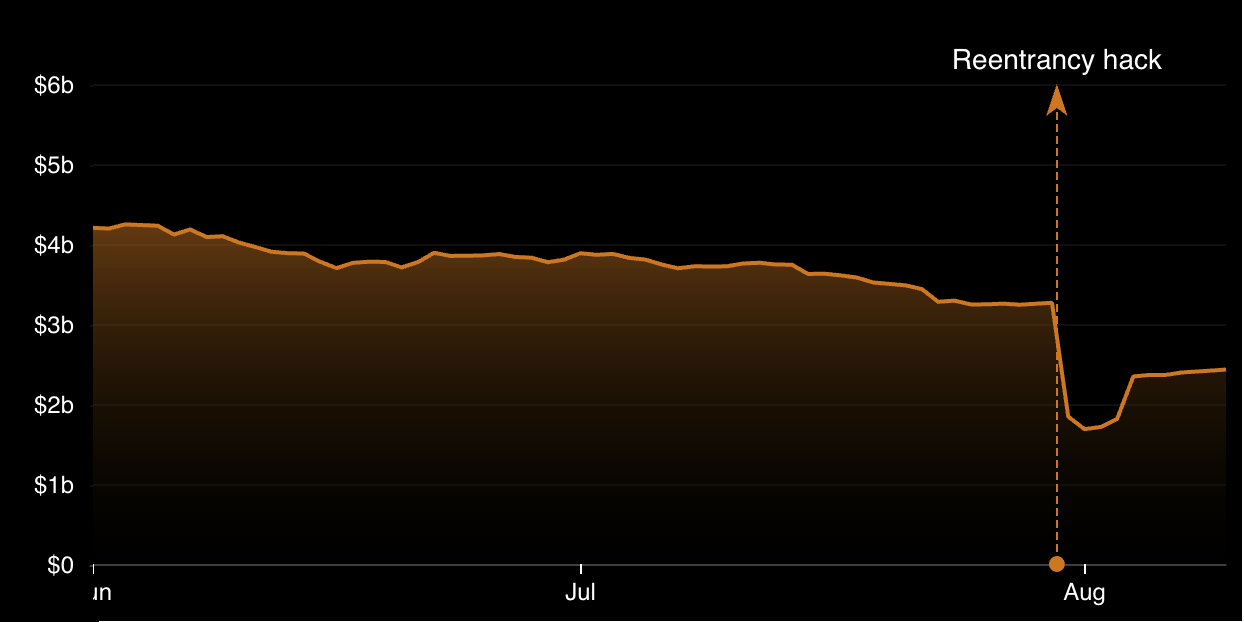
\includegraphics[width=\linewidth]{figs/curvetvl.png}
    %         \captionsetup{width=\linewidth}
    %         \caption{Curve's TVL following the VyperLang exploit in July 2023. Although only a handful of old pools were affected - those built on an old version of the Vyper compiler - over $\$1.5B$ USD was pulled across all pools on Curve Finance. Source: \bhref{https://defillama.com/protocol/curve-finance}{DeFiLlama}}
    %         \label{fig:curvetvl}
    %     \end{marginfigure}
        
    %     Simultaneously, we would like to minimize the ability of malicious sponsors to attack the users trading on permissionless markets. Consistent attacks on permissionless markets will damage the dYdX brand, which might have several implications for both core and permissionless markets. On Fig. \ref{fig:curvetvl}, we can see the $\$1.5$B USD drop in TVL on Curve pools following the VyperLang attack, despite only a small minority of pools being affected in the first place. That is, highly publicized attacks on permissionless markets might lead to a spread of Fear, Uncertainty, and Doubt across all dYdX v4 markets.

    %     Here we dive into the details of permissionless listings. We aim to provide a detailed overview of the design space surrounding permissionless listings. We hope this elucidates the challenges and potential solutions for implementing permissionless listings following the launch of dYdX v4.

    %     \subsubsection{Listing Fees}

    %         Listing fees, similar to those on Osmosis, are meant to prevent frivolous listings. Frivolous listings hog the protocol’s resources, and generally create more clutter for traders to sift through. The fee should then be thought of as a “Pigouvian tax” on market listings, calibrated against the marginal cost incurred by the protocol for every market listing. 

    %         Naturally, the fee might be denominated in DYDX, where the market's sponsor burns some amount in DYDX token to list the market. In theory, this value is then distributed amongst all token holders, including the stakers and validators that incur the additional costs of supporting new markets. Alternatively, this listing fee might be sent to the community treasury, which the community may then use for discretionary efforts. A recent \bhref{https://forum.osmosis.zone/t/proposals-addressing-scam-pools-increase-the-pool-creation-fee/42/4}{proposal} on Osmosis goes over how this listing fee may be used to fund initiatives to identify and close predatory pools. 

    %         We might begin with a listing fee of 100 DYDX, or approximately $\$200$ USD, and increase or decrease it depending on the rate of new market listings. Of course, this fee must be calibrated against large movements in the price of DYDX.

    %         As we will discuss, we might implement additional constraints around market listings. For this reason, we might avoid needing a listing fee altogether.
            
    %     \subsubsection{Sponsor Bonds} \label{subsubsec:bond}

    %         Following conversations with several community members, we consider the use of bonds as a deterrent to malicious market listings. A Sponsor might be required to deposit a minimum bond to list a permissionless market, such as $\$10K$ USDC. Governance may then slash the newly listed market if it determines that the sponsor has misbehaved. Ideally, this would prevent Sponsors from listing markets with tampered oracles or manipulable token supplies. New Sponsors might choose to bond into the market to receive Sponsor Rewards, which we discuss below. Depending on how these bonds may be claimed back by the Sponsors, we might require that permissionless markets hold a minimum bonded amount, otherwise they are placed in close-only mode.

    %         In the remainder of this section, we discuss the potential design of this bond.

    %         \textbf{Bond Denomination}

    %         Two natural choices arise for the denomination of the sponsor bond: USDC and DYDX. Denominating the bond in DYDX adds additional utility to the DYDX token, but detracts from the proof-of-stake security of the blockchain: the less DYDX is available to stake and secure the chain, the more vulnerable the chain is to a hostile takeover. Depending on the size requirements for a Sponsor bond, this might or might not be a concern. Furthermore, the bond is serving as risk capital for the collateral being traded in the market, currently denominated in USDC. If DYDX depreciates relative to USDC, then an attack on the market that takes some or all of this collateral might suddenly become profitable for the Sponsor, despite them losing their bond.
            
    %         Denominating the bond in USDC removes this security-dependency on DYDX price. It also enables an interesting synergy: we may allow the liquidation engine to trade against the Sponsor's bond. That is, the profit or loss from a liquidation in the permissionless market is counted towards or against the Sponsor's bond. We will discuss this liquidation fund idea below. 
            
    %         \textbf{Slashing}

    %         The bond primarily serves as collateral that governance may slash if a market listing is found to be malicious. It can be understood as a temporary, market-specific safety module. Once slashed, the bond may accrue to the communtity treasury, and may then be used to make traders in the market whole or aid in other efforts to mitigate damage from the attack. We cannot exhaustively enforce all the conditions under which governance may slash a bond. However, part of the permissionless listings design should be to clearly define conditions for slashing. We consider a few clear candidates:

    %         \begin{enumerate}
    %             \item Oracle or price manipulation attacks.
    %             \item Listing “blacklisted” markets. For example, dYdX governance may opt to blacklist markets that pose some legal or regulatory concerns.
    %         \end{enumerate}

    %         \callout{[DRC] Slash XYZ Market Bond}{Recently, traders and market makers in the XYZ-PERP market have been attacked. A trader took a large SHORT position in the XYZ-PERP market, and shortly thereafter the price plummeted from $\$5$ USD to $\$0$ USD in the span of a few hours. Before the attack, the market had a net open interest of $\$100K$. Upon investigation, we have found that <explanation of attack>. This proposal aims to slash the USDC that was bonded into the XYZ-PERP market and disburse it \textit{pro-rata} to traders and market makers that lost money in the attack.\vspace{0.25cm}

    %         \begin{center}
    %             \textbf{Voting}
    %         \end{center}
            
    %         \begin{itemize}
    %             \item \textbf{YAE.} Slash XYZ-PERP bonds and and disburse them \textit{pro-rata} to victims of the attack.
    %             \item \textbf{NAE.}
    %         \end{itemize}}

    %         \textbf{Withdrawing}

    %         If a bond is not slashed it must somehow be claimed back by the Sponsor. There are several ways this might be implemented. Below is a non-exhaustive list:

    %         \begin{enumerate}
    %             \item Bonds can only be claimed once a market is upgraded or abandoned. This incentivizes Sponsors to list liquid and active markets that may quickly be put up for an upgrade. However, this likely places too much risk on the Sponsor, since there is no guarantee for when the bond may be withdrawn. 
    %             \item Same as above, but the bond can be traded in an open market. For example, a Sponsor may list or bond into a permissionless market and trade the claim on their bond. As we will discuss below, bonding into a market may be imbued with Sponsor incentives, such as getting a cut of the trading fees. The original Sponsor might decide to exit their position as the Sponsor of the market, and sell it to another Sponsor who is willing to risk the time it takes to upgrade or abandon the market (potentially via an auction). For example, the original Sponsor might have bonded $\$8K$ USDC, accrued $\$2K$ in rewards, and then sells their position for $\$9K$, paying a $10\%$ liquidity premium. This is effectively how bond markets in traditional finance work. 
    %             \item Bonds can be claimed with a fixed cooldown period. If no other Sponsor bonds into the market and the remaining bond is claimed, the market is abandoned (e.g., put into close-only mode). However, as the cooldown approaches expiry, the market becomes much riskier: the sponsor may attack the market and claim their bond before governance has the time to go through an on-chain proposal to slash it. In this case, traders in permissionless markets must be made aware of the evident risk that a market with an expiring bond is much less secure.
    %         \end{enumerate}

    %         Although option (1) prioritizes the security of the market (i.e. preventing a market from having open positions, but not bond at risk) it might be too prohibitive for Sponsors. Option (2) somewhat addresses this concern by allowing Sponsors to trade their bonds in a market, potentially implemented using the x/NFT module on the CosmosSDK, but this might be an over-engineered solution for a relatively small and niche market of Sponsors. Option (3), although it sacrifices some security assumptions, would be the least prohibitive, and potentially simplest solution for Sponsors to list new markets. It would, however, place some burden on traders to be aware of potential bond expirations. We discuss the length of this cooldown period in the bond sizing segment below.

    %         \textbf{Liquidations and Deleveraging}

    %         If permissionless markets do not have access to the global insurance fund, then how may we ensure timely liquidations of unprofitable positions? Two ideas might come to mind. The first, alluded to previously, is using a Sponsor's bond as a potential insurance fund for the market. This places significant risk on the Sponsor, who might then be discouraged from listing a market altogether. Especially in nascent, volatile markets, expecting any Sponsor to bear the entire risk of liquidations in the market might be a tall ask. Data on the profitability of liquidations on dYdX v3, and potentially on the dYdX v4 testnet, could help determine whether this risk is prohibitive for Sponsors. Furthermore, a Sponsor might find clever ways to wash trade such that unprofitable liquidations accrue to the Sponsor herself. 

    %         Instead, an ``auto-deleveraging'' approach might be the base-case for permissionless markets. Deleveraging is implemented on a number of futures exchanges, and was \bhref{https://help.dydx.exchange/en/articles/4797358-contract-loss-mechanisms}{implemented} as a last-resort tool for liquidations on dYdX v3, in case the insurance fund was depleted. Auto-deleveraging entails offsetting losses from unprofitable positions against the profit from the most profitable, and highest leverage positions.\sidenotequote{In the event that the insurance fund is depleted, positions with the most profit and leverage may be used to offset negative-balance accounts, in order to maintain the stability of the system.}{\bhref{https://help.dydx.exchange/en/articles/4797358-contract-loss-mechanisms}{dYdX Help Center: Contract Loss Mechanisms}}

    %         Furthermore, auto-deleveraging might itself be a line-of-defense against malicious Sponsors. When a Sponsor lists a malicious market, they profit by opening positions and manipulating oracle prices in their favor. Their profit is contained within the permissionless market until they withdraw it. Presumably, an auto-deleveraging scheme would claw back a portion of these profits at the same time that counterparties become liquidatable: mitigating the incentives for attacking the market. Depending on how withdrawals and auto-deleveraging are implemented in dYdX v4, this could be a significant deterrent against malicious permissionless listings.

    %         \textbf{Sponsor Rewards}

    %         Sponsoring a permissionless market with a bond incurs a significant cost-of-capital on behalf of the Sponsor. Sponsors might have some intrinsic incentives to list new markets: they might be a Market Maker looking to capture the spread in trades on this new market, or a DAO trying to increase the visibility and attractiveness of their token. However, additional incentives, or Sponsor Rewards, might help in making the permissionless listings market more competitive, and therefore better at identifying new and emerging markets. The incentives would encourage new Sponsors to bond into existing permissionless markets, bolstering their security assumptions (i.e. there is more capital at risk) and helping traders identify which markets are legitimate. 

    %         These incentives might be, for example, that some percentage of trading fees in the market are disbursed \textit{pro-rata} amongst the Sponsors. We assume this does not incentivize validators to censor transactions from permissionless markets due to lower fees, since they may be subject to social slashing for doing so. Notice that if this is implemented, denominating the bond in DYDX would directly detract from the security of dYdX chain since there would be an alternative source of yield for DYDX holders. 
            
    %         However, if rewards for sponsoring permissionless markets are too attractive, then we create perverse incentives for Sponsors, who might often be market makers or token holders, to keep permissionless markets from being upgraded. In order to expedite the upgrade or abandon process, one solution might be to lock the Sponsor's rewards until the market is upgraded or abandoned.

    %         \textbf{Sizing Bonds and Sponsor Rewards}

    %         Sizing the bond will be a balance between minimizing the barriers to list legitimate market and mitigating the frequency of and damage caused by malicious listings. Some simple solutions might be to choose a relatively high minimum bond to minimize scams early into the permissionless listings program, and gradually reduce the bond size and observe whether there are meaningful increases in legitimate or malicious listings. Another option is to simulate the size of potential attacks on permissionless markets and set the minimum bond to be equal to that expected value.

    %         One possible heuristic is to consider the implied ``Sponsor Risk Premium'' for listing new markets. Assuming a risk free rate of $5\%$ and a minimum bond size of $\$100k$ USD, a Sponsor effectively pays $\$5K$ USD per year in opportunity cost for listing the market. This is a very small amount. If we assume a cooldown period of 1 month to withdraw the bond, the Sponsor is paying an opportunity cost of $\approx \$420$ USD for listing the market. If the Sponsor is rewarded with, say, $10\%$ of the trading fees in the market where taker fees are 5bps, then even a relatively small monthly volume of $\$8M$ USD would be required for the Sponsor to break even. We note that all markets on dYdX v3 exhibit significantly more volume than $\$8M$ USD a month. Given empirical data on trading volume, we might reverse engineer a reasonable bond to require from Sponsors as well as the percentage of trading fees they receive.

    %         With this approach, the Sponsor is incentivized to list popular markets to obtain enough rewards to offset their cost of capital. If these rewards are only unlocked if the market is upgraded, then we mitigate the incentives that Sponsors have to keep markets from being upgraded, as well as the incentives they might have to attack the market and risk both their bond and their rewards.

    %         \textbf{Open Interest Caps}
            
    %         We may additionally consider that the Sponsor's bond caps the amount of open interest available in the permissionless market. For example, the cap on open interest might be 100x the amount currently bonded into the market. If open interest exceeds this cap, then the market is placed into close-only mode. This both caps the maximum upside an attacker can get from manipulating the price of the underlying token, and creates clear utility for new Sponsors to bond into the market, and take a cut of the additional trading volume that they enable. 

    %         \textbf{Oracles}

    %         Finally, the initial design for permissionless listings might require whitelisted oracles. For example, dYdX v4 is launched with a set of oracles that Sponsors can use to list new markets, and governance controls these oracles. To a certain extent, this might itself invalidate the idea that the markets are ``permissionless'', since new projects would have to submit a DIP to be included in the list whitelisted oracles. \sidenotequote{here are two unique price oracles used by SynFutures: Chainlink and LWAP (liquidity-weighted average price) from spot DEXs. If an asset is not native to the chain with SynFutures, the Chainlink oracle is used. If the asset is native, SynFutures uses an LWAP from spot DEXs. The LWAP oracle calls for pricing data from DEXs where the target asset is listed and assigns a weight to them based on the DEXs’ liquidity. With both oracles, there is a maximum spot index price movement of 1\% per minute. This smoothing mechanism is used to minimize the impact of price manipulation on the spot DEXs since the mark price which is used to calculate the unrealized PnL of positions follows the spot index price.}{\bhref{https://messari.io/report/synfutures-the-permissionless-trading-solution-for-crypto-assets}{SynFutures: The Permissionless Trading Solution for Crypto Assets}}

    %         Other guardrails may be placed on oracles instead. For example, oracle updates may be smoothed such that prices reflected an exponential moving average, or prices themselves cannot change by more than a certain percentage per block. This added complexity might help mitigate the damage from price manipulation attacks, but wouldn't solve them entirely

    % \subsection{Next Steps}

    %     Permissionless market listings are a massive undertaking on dYdX v4. This section kicks-off the conversation for the community on the trade-offs with permissionless listing designs, but does not provide an opinionated proposal. In Fig. \ref{fig:permlistings}, we go over an example for what permissionless listings might look like, to consolidate the reader's understanding of the design space.

    \subsection{Summary}

        Permissionless listings are one of the most exciting innovations of dYdX Chain, and have been instrumental in the growth of several other DeFi protocols including Uniswap and Osmosis. With permissionless listings, dYdX v4 may scale from 32 initial markets to hundreds of new derivative markets with little to no governance overhead. This, in turn, could lead to a 10x increase in trading volume and fees.

        On the other hand, permissionless listings also have some undesirable implications for the protocol, including tampered market listings and the fragmentation of liquidity. Given the complex machinations of a cross-margined perpetuals exchange, we must consider:
 
        \begin{itemize}
            \item Will permissionless markets have isolated collateral?
            \item Will permissionless markets have isolated insurance funds?
            \item Will permissionless markets be eligible for Trader Rewards and Market Maker Rebates?
            \item Will permissionless markets have permissionless incentives?
            \item What preventative mechanisms will be established to prevent attacks on permissionless markets?
        \end{itemize}

        In Fig. \ref{fig:permlistings}, we provide an example for what the permissionless listings process could look like. We consider requiring a ``bond'' from the market Sponsor that governance may slash if the market is listed with a tampered oracle or token supply. This bond acts as a disincentive to list tampered markets due to the risk of slashing.  
        
        \begin{figure*}[htp]
            \centering
            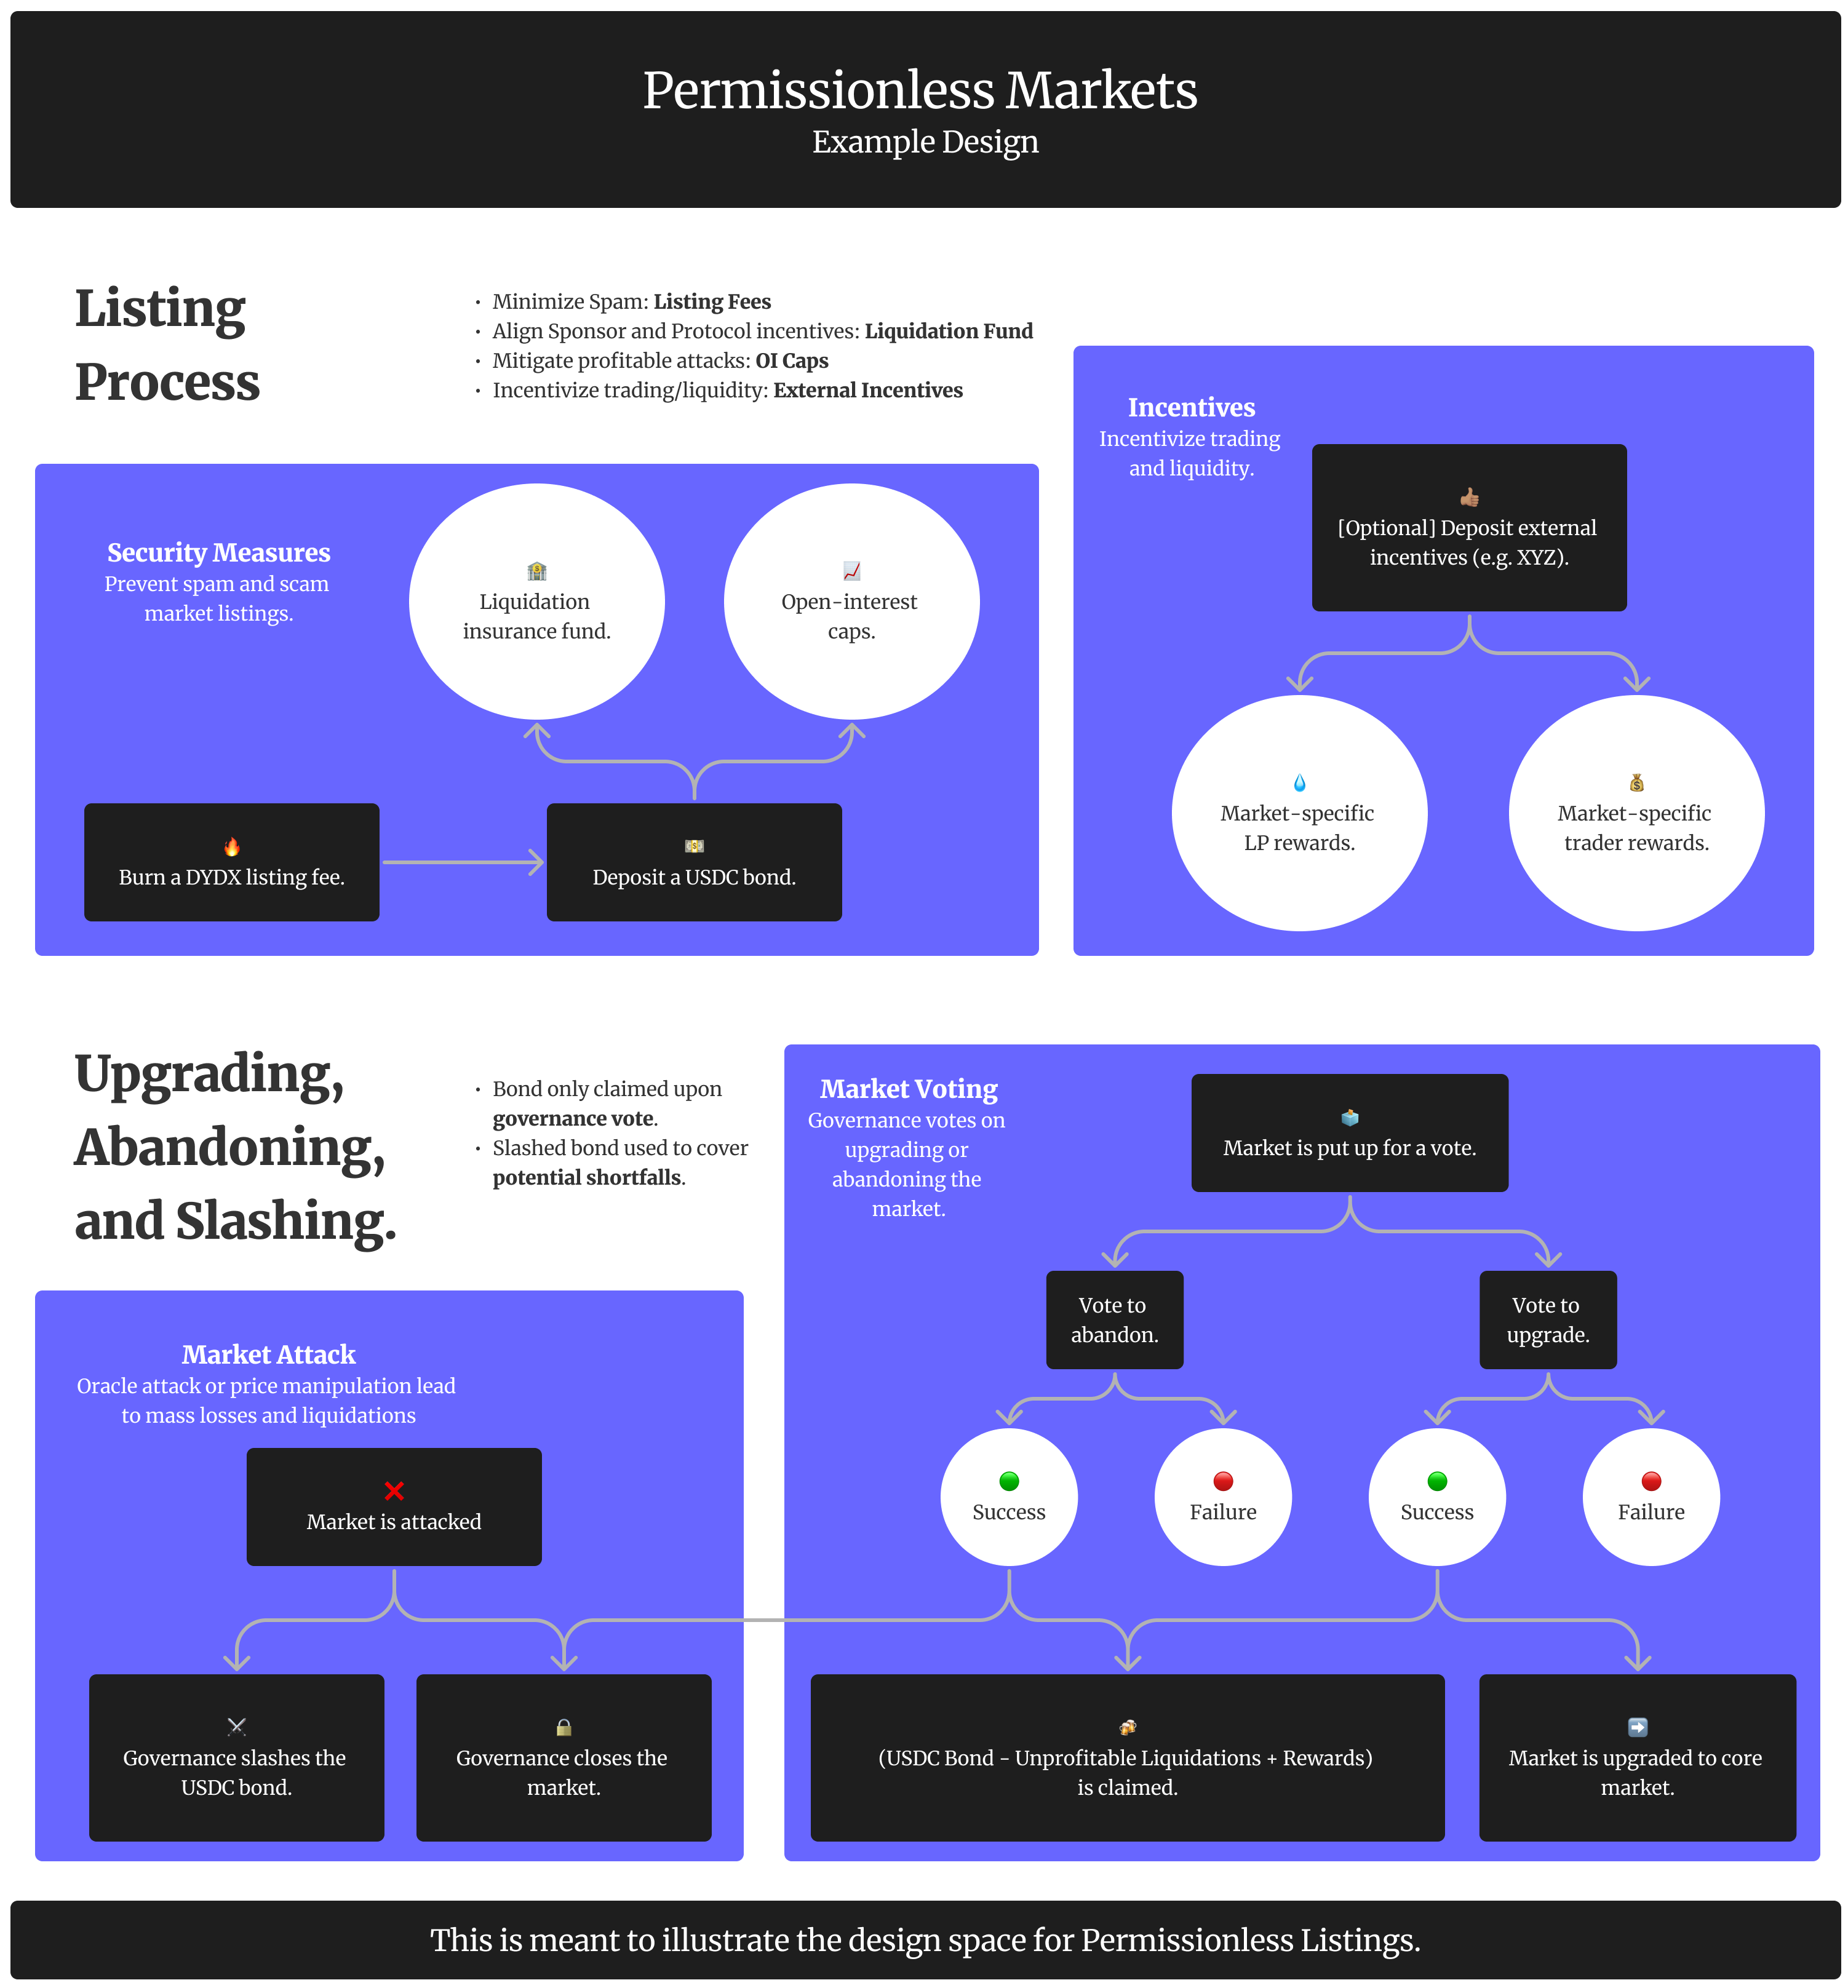
\includegraphics[width=0.95\linewidth]{figs/Permissionless Market Listings.png}
            \captionsetup[]{width=0.95\linewidth}
            \caption{Permissionless Listings, example.}
            \label{fig:permlistings}
        \end{figure*}